
%V
\section{Synthèse des performances réalisées par le modèle multiphysique $\mathrm{n}^{\circ} 2$ et évolution du prototype (ou dispositif expérimental) du Sled $0,3 g$ \label{ccs_mp_2022_sec_5}}

L'objectif est à présent de fournir aux ingénieurs une synthèse du travail réalisé et à poursuivre.

\ifprof
\else


Plusieurs simulations ont été réalisées avec le modèle multiphysique $\mathrm{n}^{\circ} 2$ pour différentes masses de passagers potentiellement embarqués de 30 à 150 kg . Les résultats sont présentés en figure \ref{ccs_mp_2022_fig_19}. Seule la première partie de la courbe de simulation d'un cycle complet est représentée. Elle correspond à une accélération constante $a_{c}=+0,3 g$ pendant 1 seconde.

\begin{figure}[!h]
\centering
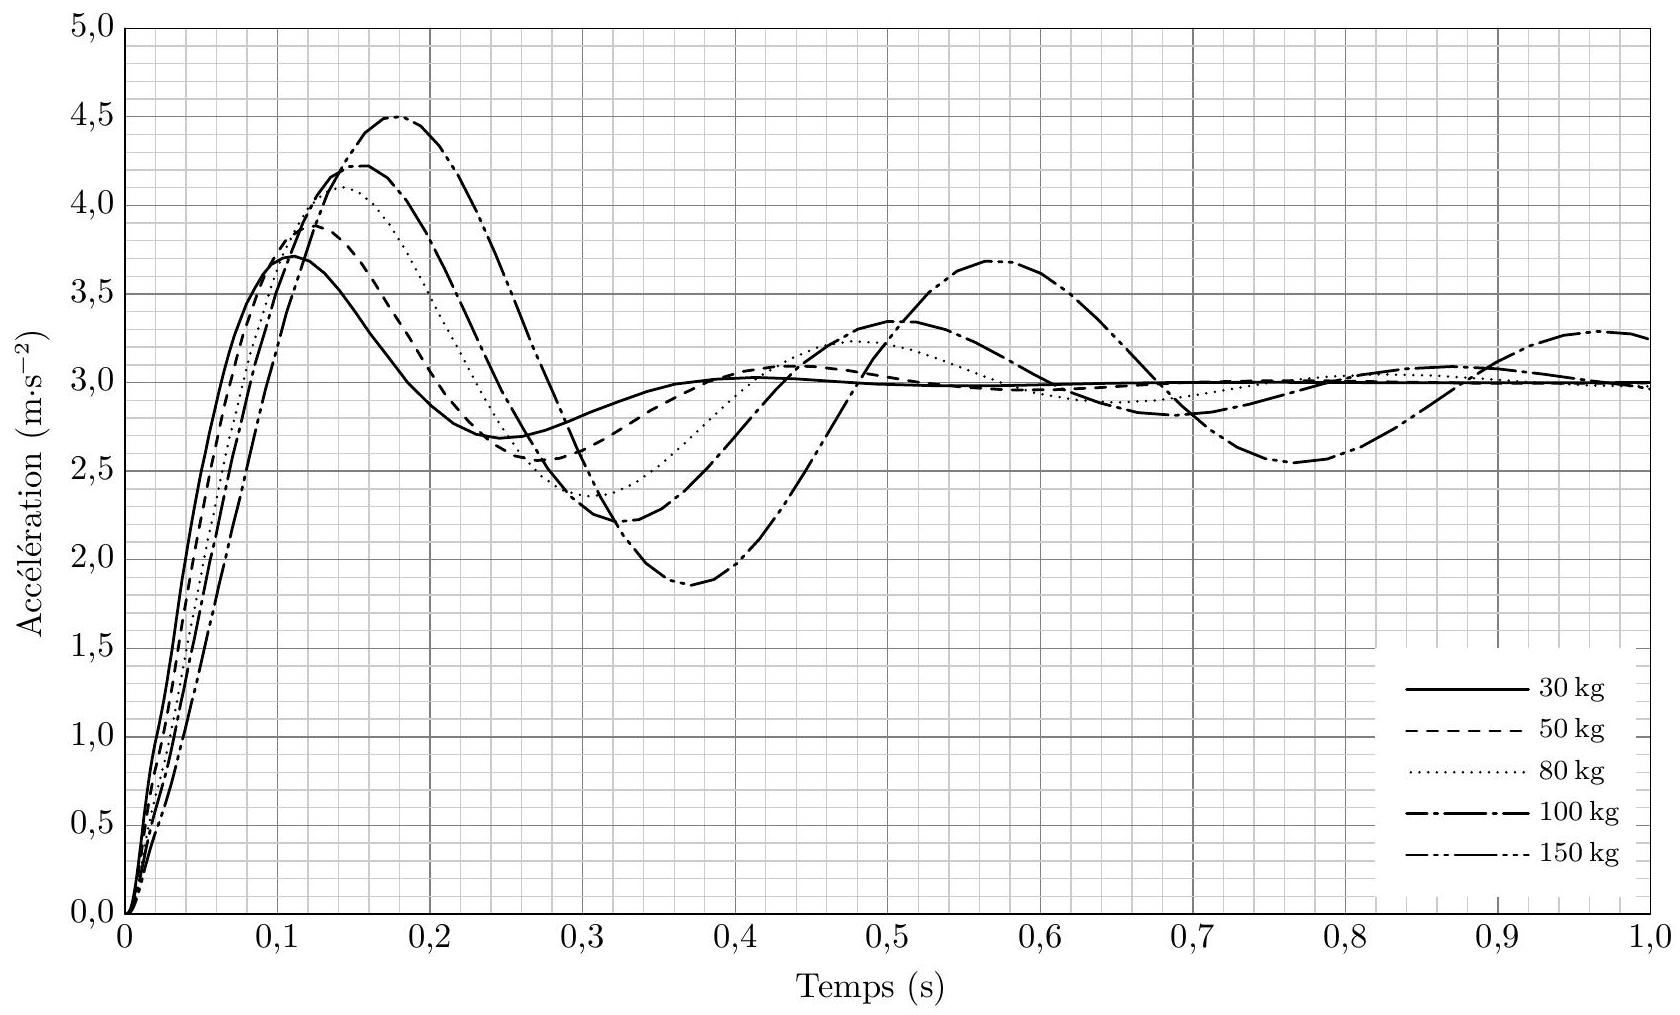
\includegraphics[width=\textwidth]{2025_07_06_ec63d2f3afc18cdeeb83g-14}

%Figure 19 
\caption{\label{ccs_mp_2022_fig_19}Simulations du modèle multiphysique $\text{n}^{\circ} 2$ pour différentes masses de passagers}
\end{figure}
\fi

%Q 47. 
\question{\label{ccs_mp_2022_sec_q_47}À partir de la figure \ref{ccs_mp_2022_fig_19}, parmi les exigences vérifiables, identifier et lister celles qui ne sont pas validées. Préciser, pour chacune d'elles, à partir de quelle valeur de masse ces exigences ne sont plus vérifiées.}
\ifprof
\begin{corrige}
\begin{itemize}
\item \texttt{Id : 1.1.1.1.1} : $M G < 7$ dB et $M P > 30\degres$. Cette exigence ne peut pas être vérifiée à l'aide de la \textsc{Figure} \ref{fig:sled19}.\\

\item \texttt{Id : 1.1.1.1.2} : le premier dépassement doit être inférieur à $20\%$. On observe alors sur la \textsc{Figure} \ref{fig:sled19} :

	\begin{itemize}
	\item $30$ kg : $\dfrac{3.7-2.94}{2.94} \simeq 26\%$\\
	\end{itemize}

le premier dépassement de $30$ kg étant le plus faible, l'exigence n'est donc pas validée.\\

\item \texttt{Id : 1.1.1.2.1} : la précision doit être inférieure à $10\%$ en régime permanent :

	\begin{itemize}
	\item $150$ kg : $\dfrac{3.3-2.94}{2.94} \simeq 12\%$

	\item $100$ kg : $\dfrac{3.1-2.94}{2.94} \simeq 5.4\%$\\
	\end{itemize}

la précision augmentant avec la diminution du poids, l'exigence est validée pour les poids inférieurs ou égaux à $100$ kg.\\
 
\item \texttt{Id : 1.1.1.3.1} : l'écart relatif entre deux essais doit être inférieur à $\pm5\%$. Cette exigence ne peut pas être vérifiée à l'aide de la \textsc{Figure} \ref{fig:sled19}.\\

\item \texttt{Id : 1.1.1.4.1} : le temps de réponse à $5$\% doit être inférieur à $0.25$ s. En observant les différentes réponses temporelles de la \textsc{Figure} \ref{fig:sled19}., on remarque qu'à $0.25$ s, aucun des signaux ne respecte l'exigence.
\end{itemize}

\end{corrige}
\else
\fi

\ifprof
\else
Afin de gérer l'avancement du projet de recherche, le bureau d'études a développé un graphe d'états applicable aussi bien au dimensionnement et à la réalisation du Sled $0,3 g$ qu'à celui du Sled $1 g$ (figure \ref{ccs_mp_2022_fig_B} du document réponse).
\fi

%Q 48. 
\question{\label{ccs_mp_2022_sec_q_48}Retracer le parcours effectué dans cette démarche de conception en repassant en couleur, sur la figure \ref{ccs_mp_2022_fig_B}, les liens concernés et entourer la situation dans laquelle se trouve l'avancement actuel du projet de Sled $0,3 g$.}
\ifprof
\begin{corrige}
\end{corrige}
\else
\fi

\ifprof
\else

\begin{figure}[!h]
\centering

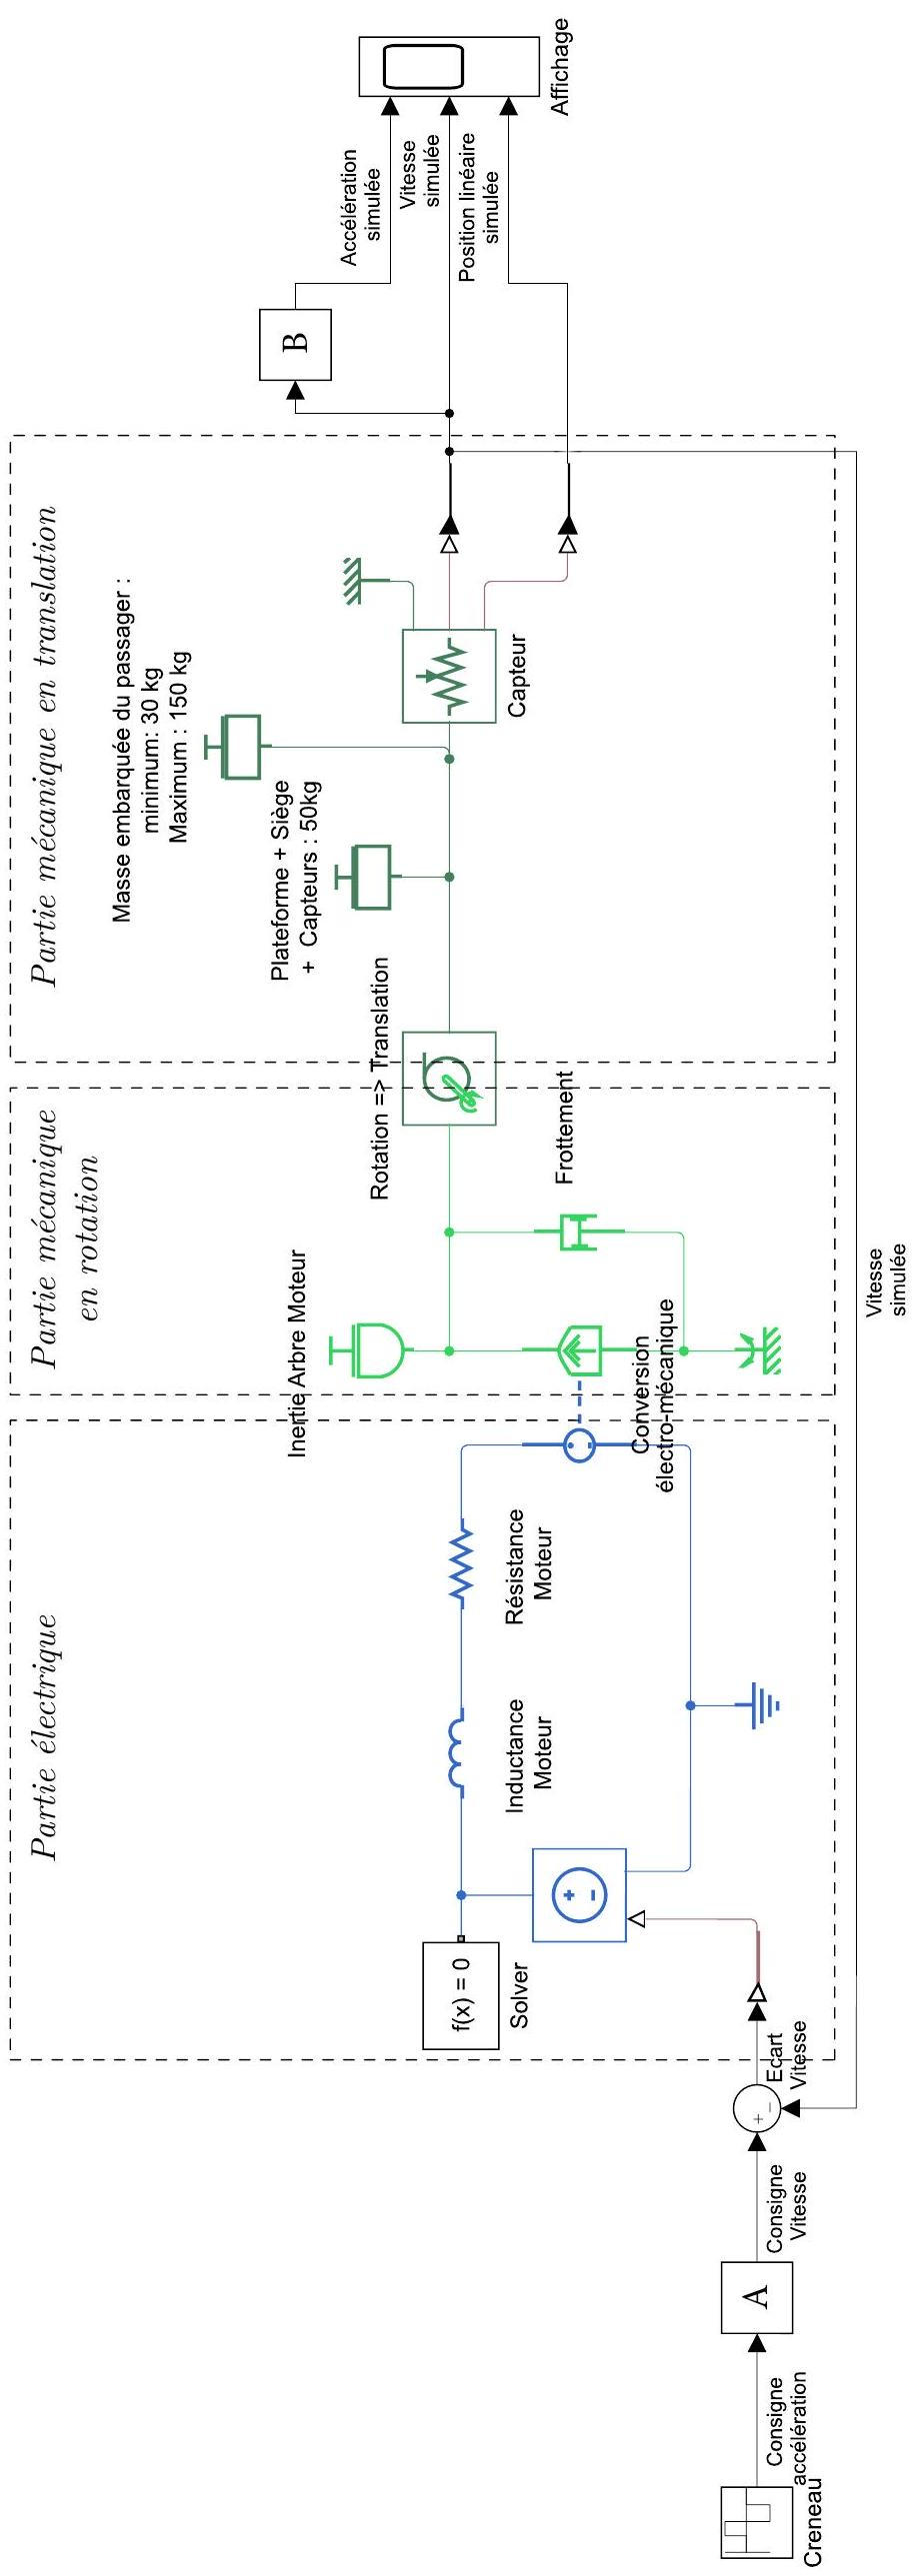
\includegraphics[height=.95\textheight]{2025_07_06_ec63d2f3afc18cdeeb83g-15}
%Figure 20 
\caption{\label{ccs_mp_2022_fig_20}Modèle $n^{\circ} 1$ du Sled}
\end{figure}


\begin{figure}[!h]
\centering
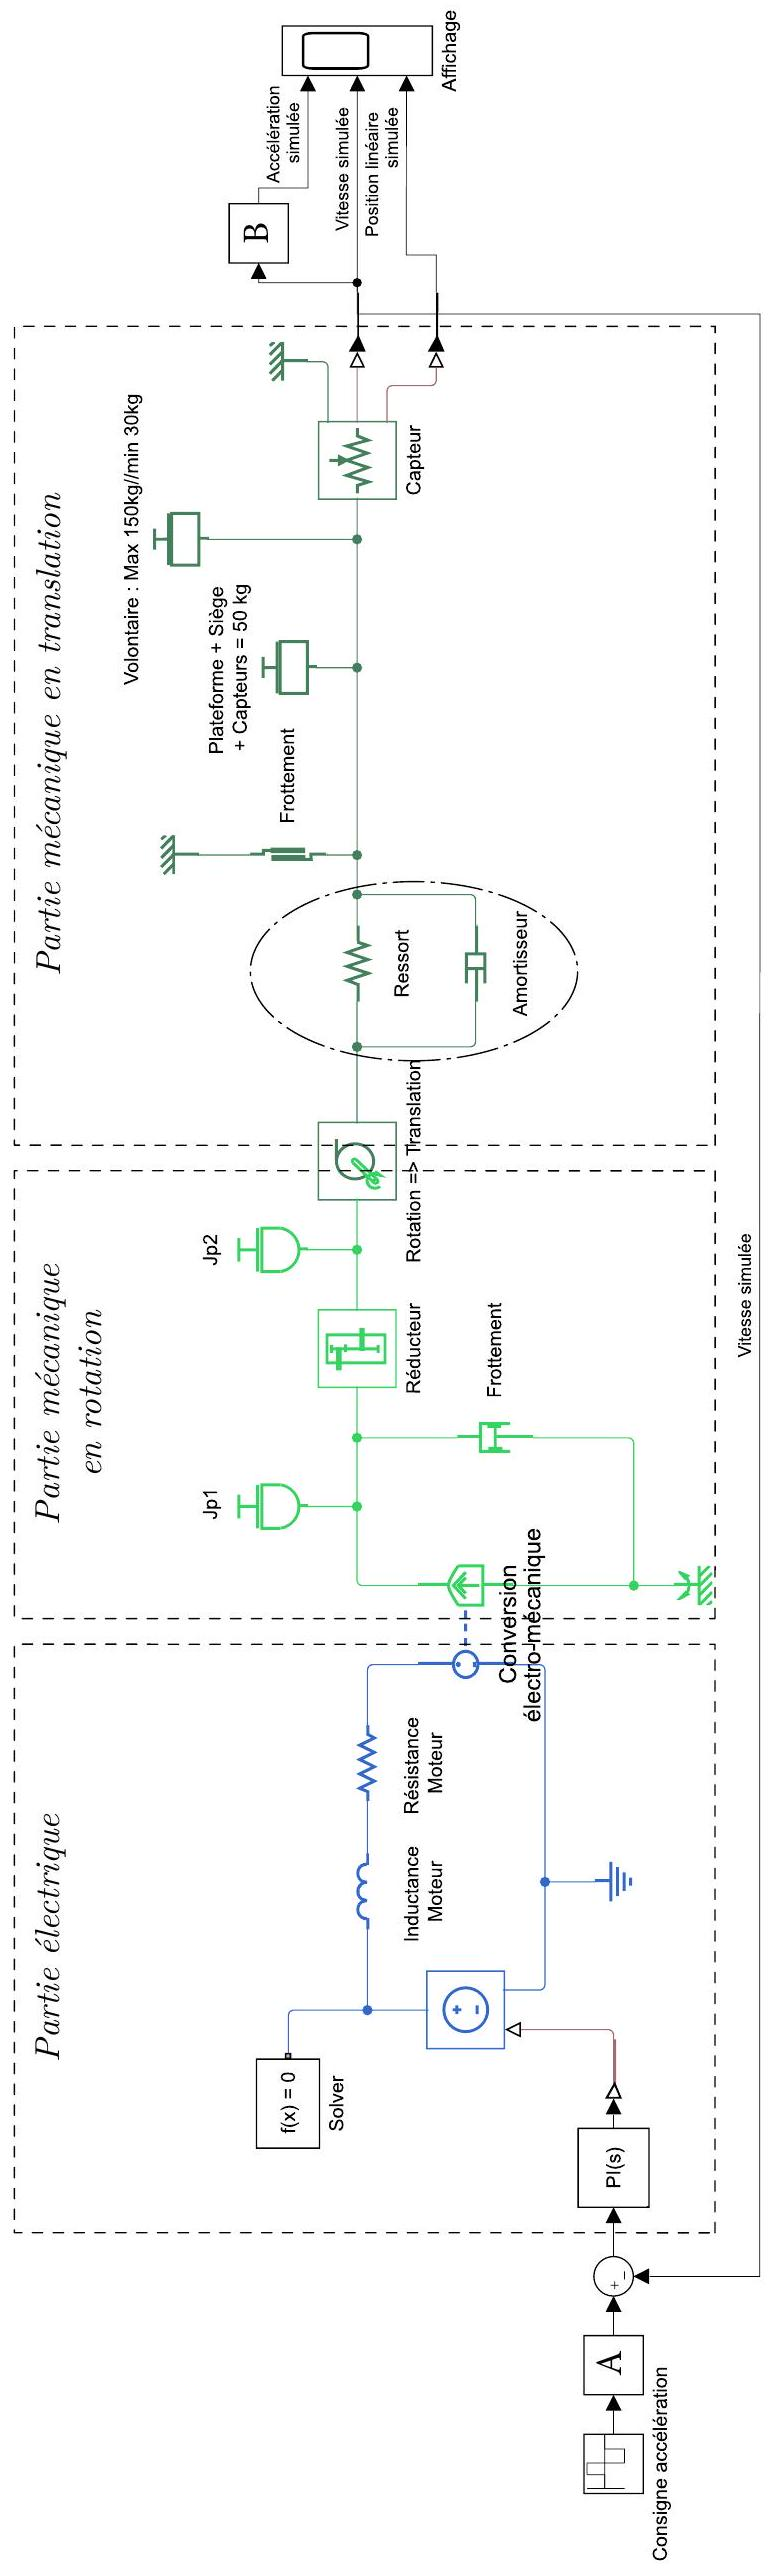
\includegraphics[height=.9\textheight]{2025_07_06_ec63d2f3afc18cdeeb83g-16}

%Figure 21 
\caption{\label{ccs_mp_2022_fig_21}Modèle multiphysique $\mathrm{n}^{\circ} 2$}
\end{figure}

\fi



\ifprof
\else
Document réponse pour l'épreuve de S2I\\

\begin{figure}[!h]
\centering
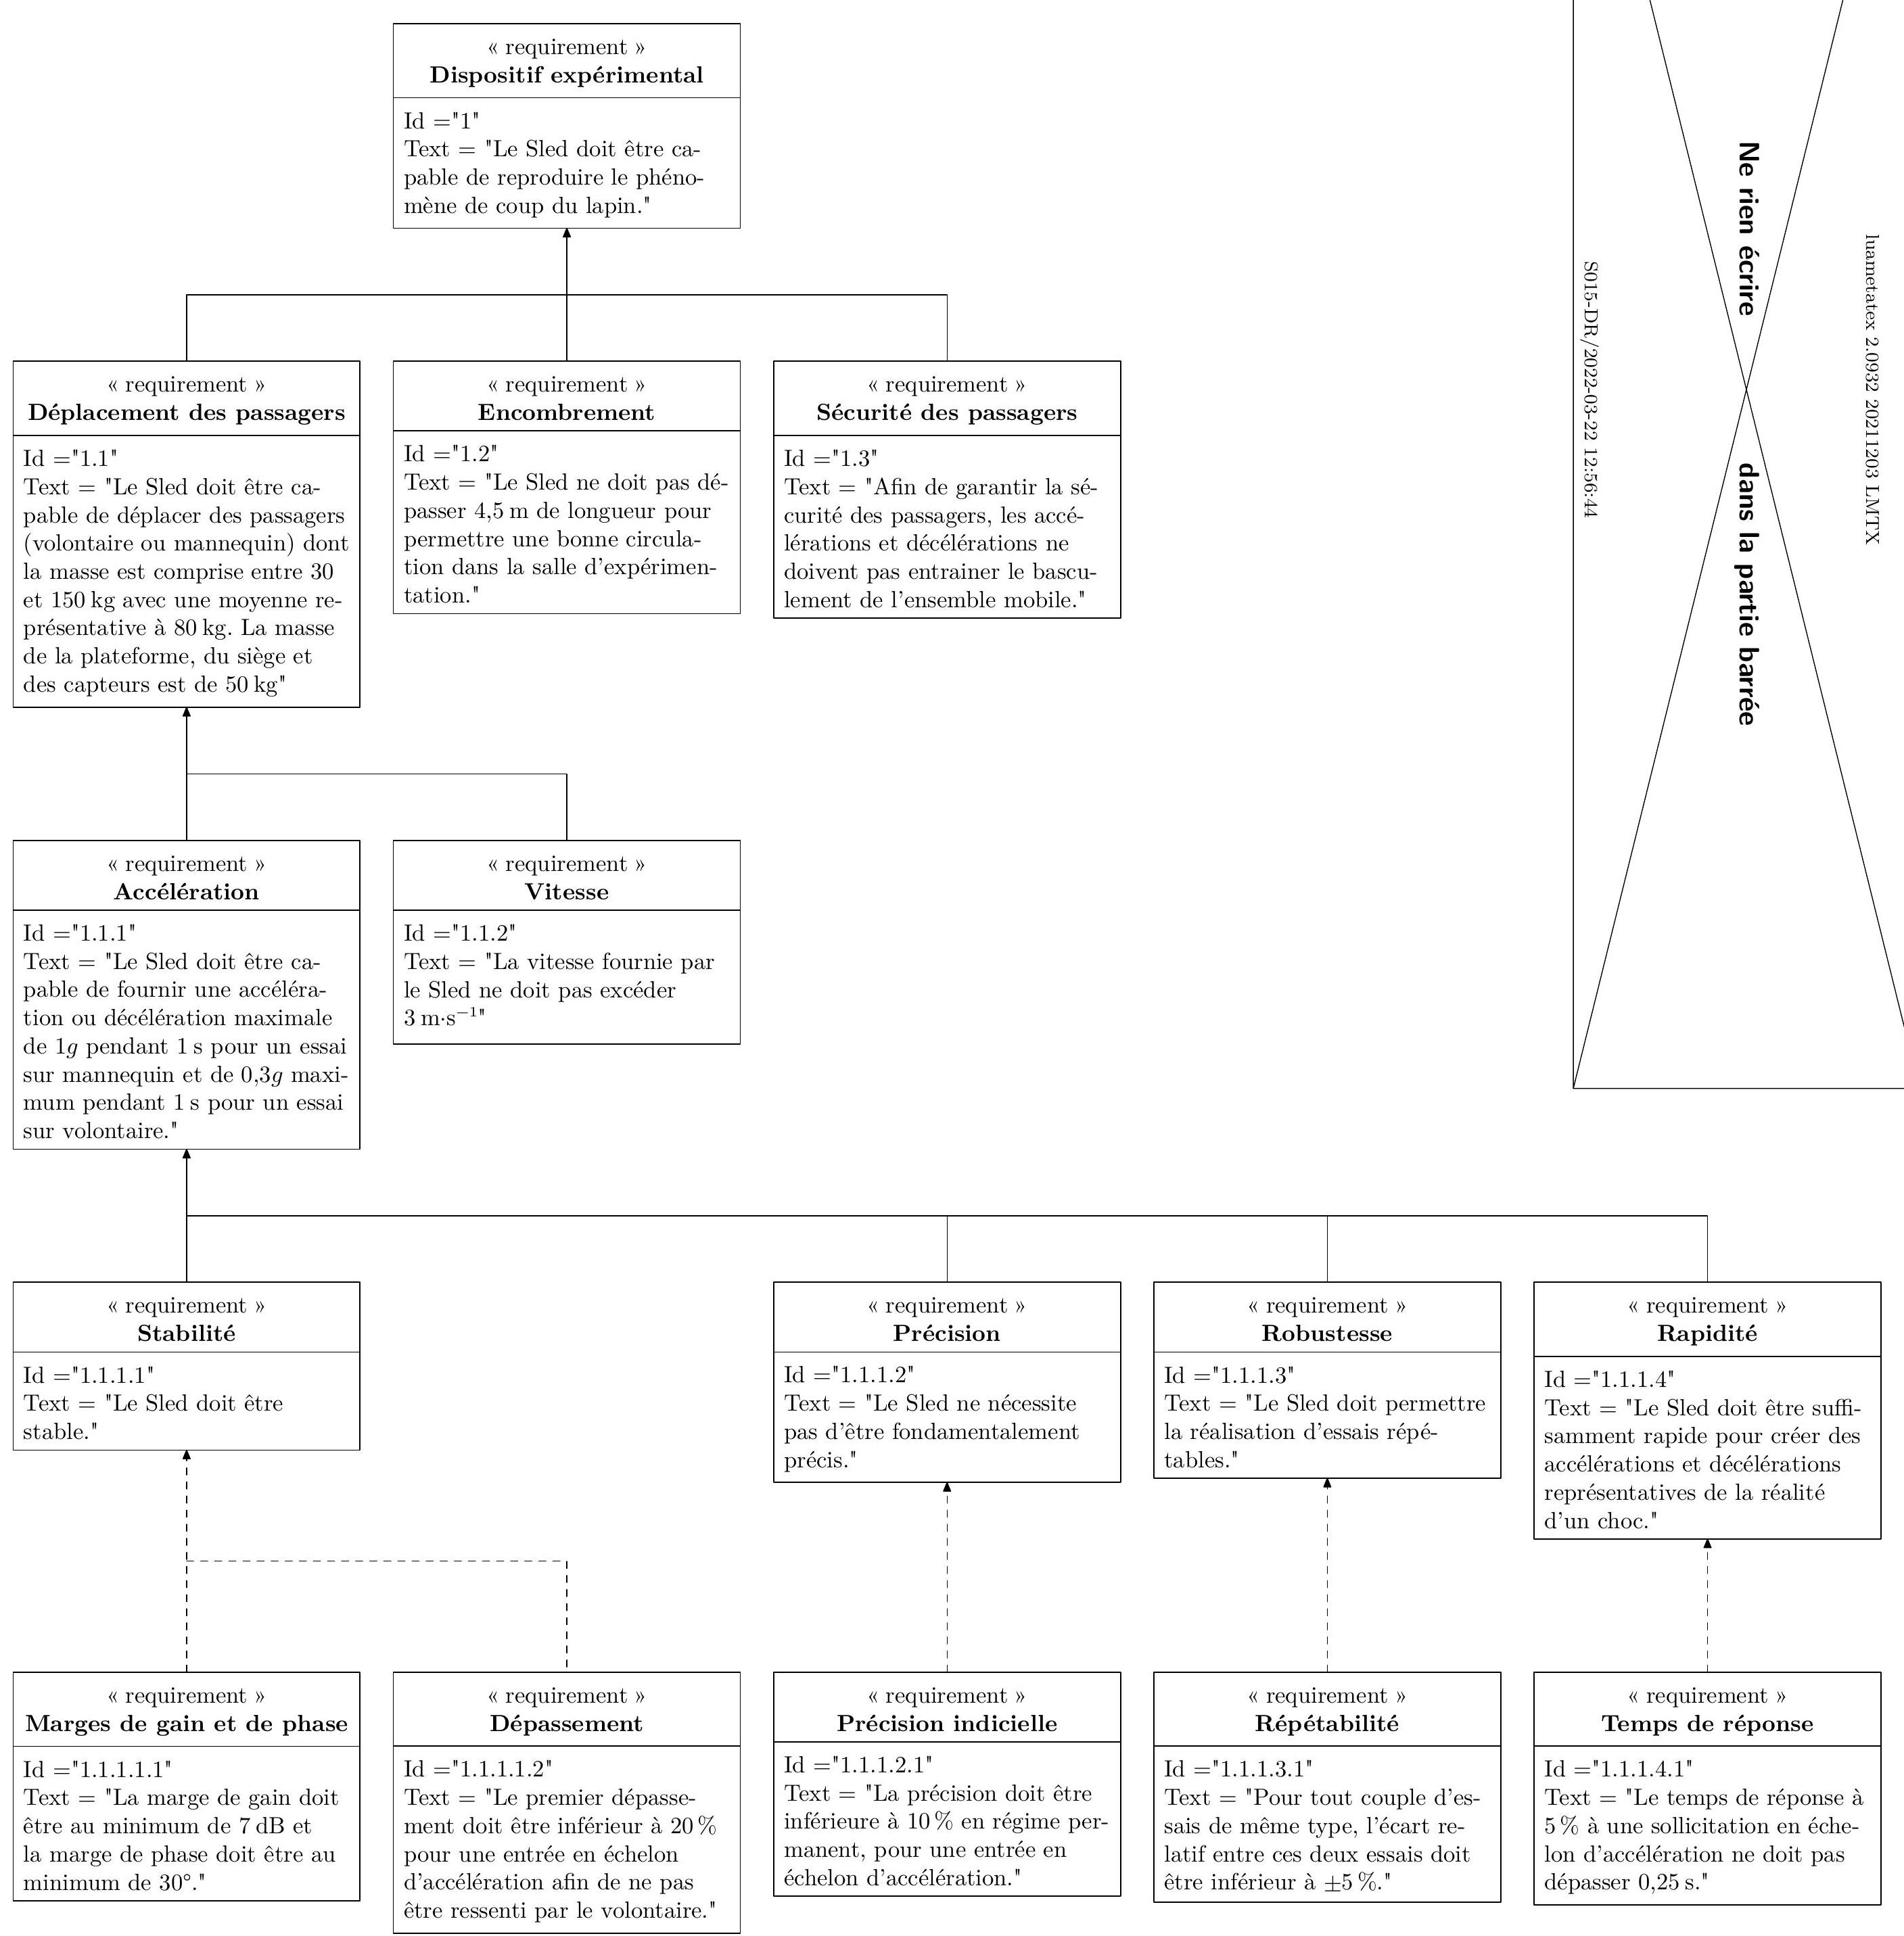
\includegraphics[width=\textwidth]{2025_07_06_ec63d2f3afc18cdeeb83g-18}

%Figure A 
\caption{\label{ccs_mp_2022_fig_A}Diagramme partiel des exigences du Sled}
\end{figure}

\section*{Question 48}
\begin{figure}[!h]
\centering

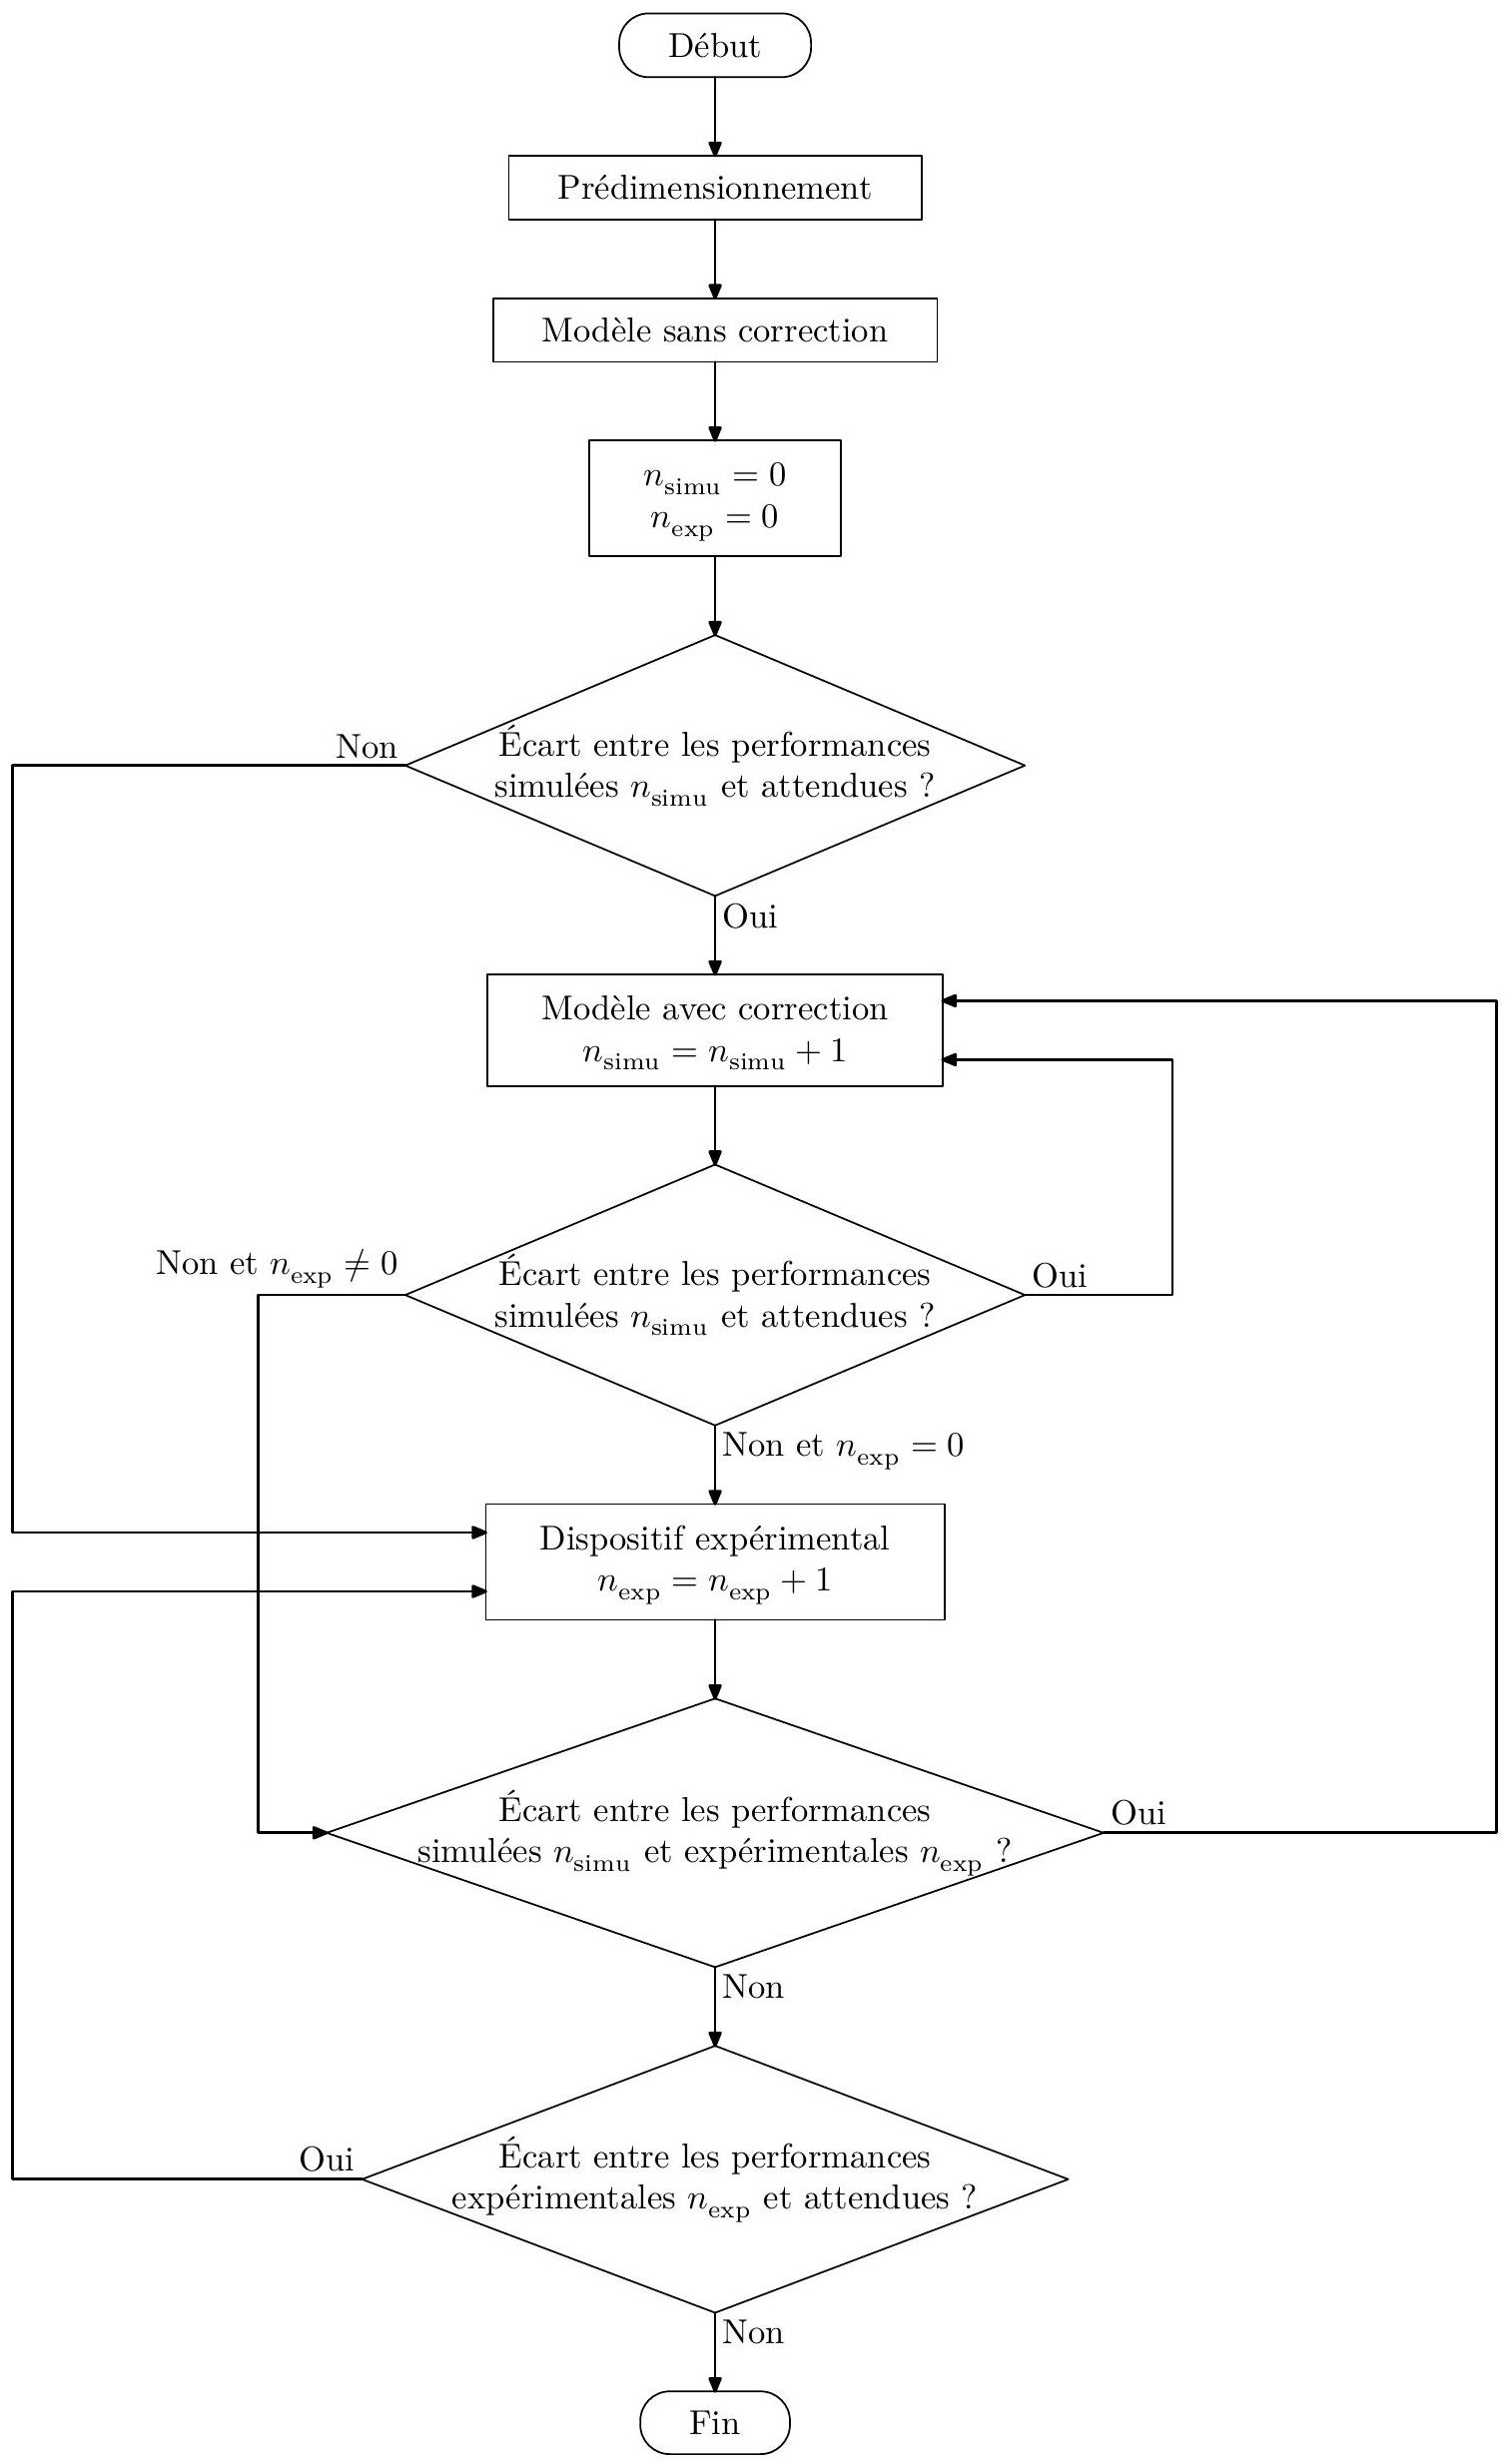
\includegraphics[width=.8\textwidth]{2025_07_06_ec63d2f3afc18cdeeb83g-19}

%Figure B 
\caption{\label{ccs_mp_2022_fig_B}Graphe d'états du projet de développement du Sled}
\end{figure}

\fi